\documentclass[review,3p]{elsarticle}
% Target: Medical Image Analysis (Elsevier). Numbers in \input{tables/...} are generated by
% scripts/make_paper_tables.py from results/ — never typed by hand.
\usepackage{amsmath,amssymb,booktabs,graphicx,xcolor,multirow,siunitx,hyperref}
\newcommand{\rev}{\textsc{rev}}
\newcommand{\ItoE}{I2E}
\journal{Medical Image Analysis}

\begin{document}
\begin{frontmatter}
\title{Where the shortcut sits: region-of-interest masking fails for in-ROI artifacts, and insertion-based erasure fixes it in dermoscopy and chest radiography}

\begin{abstract}
Medical image classifiers exploit acquisition artifacts---rulers, hair, surgical ink, chest drains---that
correlate with disease in the training data. The standard defence restricts the model to the region of
interest (ROI) by masking the background. We show that this defence is \emph{location dependent and reverses}:
it removes a shortcut that lies outside the ROI but amplifies one that lies inside it, because masking
preserves the artifact while deleting the competing evidence. We establish the effect under full control by
sweeping the artifact--ROI overlap of a synthetic artifact in dermoscopy and in chest radiography, identify
artifact \emph{retention} as the governing quantity, and confirm it on real artifacts with pre-registered
criteria: in 25,331 ISIC 2019 images masking helps against extra-lesional hair and harms against in-lesional
hair, and in NIH ChestX-ray14 lung masking cannot remove the chest-drain shortcut for pneumothorax, which lies
inside the lung field. Comparing mitigation families by the supervision they require shows that image-level
artifact labels suffice where pixel-level localisation fails (a hair detector reached IoU 0.22). Finally we
propose Insert-to-Erase (\ItoE), which needs neither localisation nor artifact labels: artifacts are
\emph{inserted}---which requires only a template library---to obtain label-independent counterfactual pairs, and
the subspace spanned by their feature differences is erased before the classifier is fitted. \ItoE{} recovers
reversed-environment performance in the in-ROI regime of both modalities without reducing clean accuracy. Code,
frozen splits and pre-registrations are public.
\end{abstract}

\begin{keyword}
shortcut learning \sep spurious correlation \sep artifacts \sep dermoscopy \sep chest radiography \sep concept erasure
\end{keyword}
\end{frontmatter}

\section{Introduction}
Deep classifiers for medical images frequently rely on features that are correlated with the label in the
training distribution but are not evidence of disease \citep{geirhos2020shortcut,degrave2021ai}. In dermoscopy,
surgical skin markings \citep{winkler2019markings} and ruler scale bars \citep{winkler2021scalebars} changed
the melanoma predictions of a market-approved system; in chest radiography, pneumothorax classifiers detect the
chest drain that treats the condition rather than the condition itself
\citep{oakden2020hidden,jimenez2023shortcuts}. Such correlations are causal in origin---suspicious lesions are
measured and marked, collapsed lungs are drained---so they are present in every retrospectively collected dataset.

The most widely recommended defence is to restrict the classifier to the region of interest (ROI): segment the
lesion or the lungs and discard the rest of the image. The rationale assumes that the shortcut lives in the
background. Rulers, hair, ink and drains do not respect that assumption. When the artifact overlaps the ROI,
masking cannot remove it; it removes everything \emph{else}. We ask whether the effect of a mitigation depends on
where the artifact sits, which quantity governs that dependence, what supervision each family of mitigations
actually needs, and whether the in-ROI regime can be mitigated without localising the artifact.

\paragraph{Contributions}
\begin{enumerate}
\item \textbf{A controlled, reversing effect.} Sweeping the overlap between a synthetic artifact and the ROI,
ROI masking changes sign: it is the best method tested when the artifact is outside the ROI and worse than doing
nothing when it is inside, in dermoscopy and in chest radiography, on general and domain foundation models.
\item \textbf{A mechanism.} Occlusion and lost context are rejected by dedicated controls; masking roughly doubles
counterfactual sensitivity to the artifact, and harm tracks artifact \emph{retention} rather than its share of the image.
\item \textbf{Confirmation on real artifacts} with pre-registered criteria: in-lesion versus extra-lesional hair
in ISIC 2019 (source-matched traps), and chest drains in NIH ChestX-ray14.
\item \textbf{A supervision-oriented comparison.} Pixel-level artifact localisation is not obtainable in practice;
image-level labels are, and they suffice; reversed-environment gains can be gamed by unpaired erasure, so they must
be read together with clean accuracy and the correlated/reversed ordering.
\item \textbf{Insert-to-Erase}, a localisation-free, label-free mitigation that works in the in-ROI regime of both modalities.
\item A reproducible protocol: leakage-safe grouped splits, pre-registration, hierarchical paired bootstrap, and
an audited public code base.
\end{enumerate}

\section{Related work}
\paragraph{Artifacts in dermoscopy} \citet{bissoto2020debiasing} annotated seven artifact types in ISIC images and
showed that debiasing is harder than it looks; \citet{nauta2022uncovering} neutralised coloured calibration patches
by inpainting and retraining---an artifact that a colour rule localises and that lies largely outside the lesion.
MaskMedPaint \citep{maskmedpaint} inpaints regions \emph{outside} the classification-relevant area. None of these
treats artifact location relative to the ROI as a variable.
\paragraph{Chest radiography} Drain-driven pneumothorax shortcuts are documented on NIH-CXR14 and CheXpert
\citep{oakden2020hidden,jimenez2023shortcuts}; recent work localises them to late layers of probed encoders
\citep{pedersen2026probes} and mitigates them by prevalence-equalised recalibration \citep{kina2026prevalence},
which requires the artifact label at test time.
\paragraph{Group robustness and erasure} Reweighting and GroupDRO \citep{sagawa2020groupdro}, last-layer
retraining \citep{kirichenko2023dfr} and linear concept erasure \citep{ravfogel2020inlp,belrose2023leace}
require artifact labels or paired data; erasure from unpaired labels removes label-correlated signal when the
concept is correlated with the label, which is why we build pairs by insertion.

\section{Problem setup and protocol}\label{sec:setup}
Let $Y\in\{0,1\}$ be the diagnosis and $A\in\{0,1\}$ the presence of an artifact. A \emph{trap} trains with
$P(A{=}1\mid Y{=}1)=0.9$ and $P(A{=}1\mid Y{=}0)=0.1$ and tests on a correlated environment with the same rates,
a \emph{reversed} environment with the rates swapped (0.1/0.9), and a clean environment without artifacts. A model
that uses $A$ gains on the correlated test and collapses on the reversed one; the primary metric is reversed-test
AUROC, and clean AUROC measures the cost of a mitigation. The overlap $r=|\mathrm{artifact}\cap\mathrm{ROI}|/|\mathrm{artifact}|$
is the controlled variable. All backbones are frozen and only linear heads are fitted (an end-to-end fine-tuning
check is reported in Sec.~\ref{sec:ft}); regularisation strength and the decision threshold (balanced accuracy)
are selected on clean validation data only. Uncertainty is a hierarchical paired bootstrap that resamples training
seeds (or cross-validation folds), then paired test images within each, computes the AUROC difference inside
each cluster and averages; predictions of different models are never pooled into one ROC curve.
Splits are grouped by lesion/patient identifier and perceptual hash.

\section{Insert-to-Erase}\label{sec:i2e}
Removing an in-ROI artifact requires its pixels; inserting one does not. Given a template library $\mathcal{T}$
(real artifact pixels transplanted from a disjoint donor pool, or a procedural generator) and a frozen encoder $f$,
every training image $x_i$ yields a counterfactual $x_i^{+}=\mathrm{insert}(x_i,t_i)$, $t_i\sim\mathcal{T}$, at a
random position that is not restricted to the background. Because insertion ignores the label, the differences
$\Delta_i=f(x_i^{+})-f(x_i)$ are independent of $Y$. \ItoE{} erases their span:
\begin{equation}
\Sigma_\Delta=\tfrac1n\textstyle\sum_i\Delta_i\Delta_i^\top,\qquad U_k=\mathrm{top}\text{-}k\ \mathrm{eigvecs}(\Sigma_\Delta),\qquad
P(z)=z-U_kU_k^\top(z-\mu),
\end{equation}
and fits the linear head on $P(f(x))$. The rank $k$ is chosen \emph{without labels} as the smallest $k$ whose
held-out paired-difference energy $\mathbb{E}\|P\Delta\|^2/\mathbb{E}\|\Delta\|^2$ falls below $0.10$ (fixed before
any experiment). Rank-1 LEACE on insertion pairs is the special case that erases only the mean shift; \ItoE{} also
erases how the shift varies with the image and the template, which is what a single direction leaves behind.
When image-level artifact labels exist, \ItoE{} composes with group-balanced reweighting.

% Results sections are generated: \input{sections/results_generated}
% Results. Every number is produced by scripts in the repository (results/SUMMARY.md, results/CROSS_COHORT.md).
% Dermoscopy results. Every number is produced by scripts in the repository; see results/SUMMARY.md.
\section{Results: dermoscopy}\label{sec:derm}

\subsection{Masking reverses with location (controlled)}
With a synthetic ruler whose overlap with the lesion is swept from 0 to 100\% (2,437 ISIC 2018 images,
DINOv2 ViT-B/14 at 518\,px, three seeds), ROI masking improves reversed-environment AUROC over ERM by
$+0.184$ [$+0.146, +0.224$] when the ruler lies outside the lesion and \emph{lowers} it by $-0.097$
[$-0.138, -0.056$], $-0.112$ [$-0.155, -0.068$] and $-0.129$ [$-0.170, -0.087$] at 50, 75 and 100\% overlap
(location interaction $+0.313$ [$+0.272, +0.353$]; Table~\ref{tab:synthetic_isic_dino518}). The sign flip is
reproduced at 224\,px ($+0.361$ at 0\%; $-0.095$ at 100\%) and under randomised ruler colour, opacity, ticks and
scale. At 0\% overlap the masked model's correlated and reversed AUROC coincide (0.849/0.849): the shortcut is
removed. At 100\% the masked model's correlated AUROC exceeds ERM's (0.961 vs 0.937): it uses the ruler \emph{more}.

\begin{table}
\caption{Synthetic ruler, ISIC 2018, DINOv2 ViT-B/14 @518: AUROC and reversed-test Δ vs ERM [95% CI]}
\label{tab:synthetic_isic_dino518}
\begin{tabular}{lllllllllll}
\toprule
Method & Needs & clean@0 & rev@0 & clean@50 & rev@50 & clean@100 & rev@100 & Δrev@0 & Δrev@50 & Δrev@100 \\
\midrule
ERM & — & 0.797 & 0.665 & 0.793 & 0.573 & 0.792 & 0.515 &  &  &  \\
ROI masking & ROI mask (train+test) & 0.849 & 0.849 & 0.829 & 0.476 & 0.825 & 0.386 & +0.184 [+0.146, +0.224] & -0.097 [-0.138, -0.056] & -0.129 [-0.170, -0.087] \\
Inpainting (oracle) & artifact pixels (train+test) & 0.810 & 0.806 & 0.809 & 0.783 & 0.807 & 0.759 & +0.141 [+0.120, +0.162] & +0.211 [+0.187, +0.234] & +0.243 [+0.218, +0.269] \\
Group-balanced & image-level A (train) & 0.814 & 0.802 & 0.815 & 0.792 & 0.806 & 0.796 & +0.137 [+0.109, +0.168] & +0.219 [+0.188, +0.252] & +0.281 [+0.248, +0.315] \\
DFR & image-level A (val) & 0.786 & 0.789 & 0.787 & 0.794 & 0.789 & 0.794 & +0.124 [+0.091, +0.160] & +0.221 [+0.184, +0.261] & +0.279 [+0.240, +0.320] \\
LEACE (paired, oracle renders) & paired renders (train) & 0.829 & 0.832 & 0.810 & 0.810 & 0.809 & 0.809 & +0.167 [+0.139, +0.197] & +0.237 [+0.212, +0.263] & +0.294 [+0.265, +0.325] \\
Repair consistency & artifact pixels (train) & 0.828 & 0.707 & 0.822 & 0.616 & 0.814 & 0.558 & +0.042 [+0.015, +0.069] & +0.043 [+0.014, +0.072] & +0.042 [+0.012, +0.073] \\
I2E (ours) & template library & 0.848 & 0.844 & 0.850 & 0.833 & 0.847 & 0.818 & +0.179 [+0.152, +0.206] & +0.260 [+0.229, +0.291] & +0.303 [+0.271, +0.336] \\
I2E + balanced (ours) & templates + A (train) & 0.841 & 0.842 & 0.843 & 0.840 & 0.844 & 0.842 & +0.177 [+0.151, +0.205] & +0.267 [+0.238, +0.298] & +0.327 [+0.293, +0.362] \\
I2E rank-1 (ablation) & template library & 0.811 & 0.799 & 0.809 & 0.770 & 0.806 & 0.730 & +0.134 [+0.115, +0.154] & +0.197 [+0.174, +0.220] & +0.215 [+0.190, +0.240] \\
Insertion augmentation & template library & 0.814 & 0.726 & 0.812 & 0.654 & 0.810 & 0.603 & +0.061 [+0.049, +0.074] & +0.081 [+0.068, +0.094] & +0.088 [+0.077, +0.099] \\
\bottomrule
\end{tabular}
\end{table}

Insert-then-erase in this table is the artifact-specific precursor of U-MtE: its insertion pairs use templates of the
artifact type (rulers) and it erases from unmasked features. U-MtE (Sec.~\ref{sec:i2e}) replaces the templates by
one generic overlay library for every modality and erases after masking; its dermoscopy results are in
Sec.~\ref{sec:solution}.

\subsection{Mechanism: retention, not occlusion or context}
Three explanations were tested separately. \emph{Occlusion}: with the ruler present but uncorrelated with the
label (50/50), masking helps at every overlap ($+0.036$, $+0.040$, $+0.039$ at 0/50/100\%); covering lesion
pixels costs nothing measurable, so the harm requires the correlation. \emph{Lost context}: dilating the mask at
50\% overlap \emph{increases} harm ($-0.097 \rightarrow -0.138 \rightarrow -0.154$ for margins 0/10/25\,px) as the
margin restores ruler pixels (retention $0.50 \rightarrow 0.73 \rightarrow 0.95$); at 100\% overlap, where retention
is already 1, harm is flat ($-0.129$ to $-0.144$) although the ruler's share of visible pixels falls threefold.
\emph{Amplified reliance}: masking doubles the same-head counterfactual sensitivity to the ruler
($|\Delta p|$ 0.235 $\rightarrow$ 0.491 at 100\%). Harm is largest for small lesions ($-0.364$ vs $+0.064$ for large
lesions at 100\%), where the ruler is a larger share of what survives the mask.

\subsection{Real hair (ISIC 2019), pre-registered}
Two traps share one hair-free group (at most 30 hair pixels): Trap~A contains hair lying mostly inside the lesion
($r\ge0.5$), Trap~B hair mostly outside ($r<0.1$); cells are matched to the hair-free source mix, and five seeds
of five-fold group-safe cross-validation give 172 reversed-test melanomas per trap. Masking helps in Trap~B
($+0.107$ [$+0.078, +0.135$]), harms in Trap~A ($-0.037$ [$-0.057, -0.019$], negative in all five seeds) and the
crossover is $+0.145$ [$+0.105, +0.181$]. The harm holds in BCN images ($-0.051$ [$-0.075, -0.027$]); in HAM it
is not distinguishable from zero ($-0.009$ [$-0.036, +0.017$]). Oracle hair inpainting helps in both traps
($+0.103$, $+0.096$). Group-balanced training and DFR, which need only an image-level hair label, give the largest
gains ($+0.225$/$+0.251$ in Trap~A, $+0.209$/$+0.215$ in Trap~B). Paired linear erasure recovers less than half of
that ($+0.086$/$+0.081$). The magnitude of the in-ROI harm depends on the definition of the comparison group: with
a looser hair-free group ($<0.1\%$ of pixels) and only heavily haired images, masking gives no benefit but no
measurable harm inside the lesion ($+0.012$ [$-0.042, +0.062$]) while still helping outside ($+0.178$); the
benefit shrinks to zero as more of the hair lies inside the lesion.

With the dermatology foundation model DermLIP, the controlled ruler sweep reverses as with DINOv2 ($+0.161$ at no
overlap, $-0.263$ to $-0.309$ at 25--100\%), but on real hair masking harms at both locations (Trap~A $-0.085$
[$-0.107, -0.063$], Trap~B $-0.088$): with this encoder masking removes disease context regardless of where the hair
lies, so no location gap appears.

\subsection{What the real-hair shortcut is made of}
Removing hair pixels at test time only closes 44--47\% of the ERM clean--reversed gap: most of what a frozen
encoder exploits in a real hair trap is not the hair pixels but what accompanies hair (hair-bearing images differ in
sex, age and body site). This bounds every pixel-level method, including oracle inpainting and U-MtE, and
explains why image-level-label methods, which remove everything correlated with the label, recover more.

\subsection{Reversed-environment gains can be gamed}
Erasing the artifact concept from unpaired image-level labels yields the largest reversed gain in the study
($+0.326$ in Trap~A) while \emph{inverting} the correlated/reversed ordering (0.618 vs 0.817). Post-hoc
prevalence-equalised recalibration \citep{kina2026prevalence} behaves the same way under the trap's 90/10 shift
($+0.427$; correlated 0.433 vs reversed 0.918). Both remove diagnosis-correlated signal or over-correct the
group prior rather than removing reliance on the artifact; we therefore read every reversed gain together with
clean AUROC and the correlated/reversed ordering.

\section{Results: ultrasound, capsule endoscopy and chest radiography}\label{sec:multi}

\subsection{Thyroid ultrasound: sonographer calipers}
TN3K images with TNCD labels (3,493 images, 1,210 malignant) carry measurement calipers that a sonographer
places on or around the nodule. Calipers were segmented by an audited rule-based detector (image-level precision
and recall 0.86--0.89). With the E13 protocol unchanged, masking the nodule helps greatly when the calipers lie
outside it (Trap~B: $+0.341$ [$+0.320, +0.363$]) and much less when they lie inside it (Trap~A: $+0.111$
[$+0.097, +0.124$]); the crossover is $+0.230$ [$+0.204, +0.255$] with DINOv2 and $+0.163$ [$+0.132, +0.194$] with
MedSigLIP. After masking, the Trap~A model still relies on the calipers (correlated 0.902 versus reversed 0.400).
With synthetic calipers swept across the nodule boundary (1,663 caliper-free images), masking gains $+0.402$
[$+0.347, +0.458$] at no overlap and $-0.030$ [$-0.079, +0.016$] at full overlap (interaction $+0.432$
[$+0.377, +0.492$]): the entire benefit of masking disappears, without significant harm.

\subsection{Capsule endoscopy: intestinal debris}
SEE-AI frames (erosion 3,550 versus polyp-like 1,931; expert lesion boxes as ROI) with contamination masks from a
patch-token probe trained on 2,160 expert-masked frames (held-out pixel accuracy 0.92, IoU 0.62). Leakage groups
are contiguous blocks of 100 frame numbers plus perceptual-hash duplicates (no video identifiers are published).
Masking helps against out-of-ROI debris ($+0.465$ [$+0.440, +0.490$]) and much less against debris on the lesion
($+0.097$), a crossover of $+0.368$ [$+0.340, +0.397$]. With synthetic debris on the 796 cleanest frames the
reversal appears: $+0.103$ [$+0.060, +0.149$] at no overlap, $-0.102$ [$-0.162, -0.040$] at full overlap
(interaction $+0.205$ [$+0.150, +0.259$]).

\begin{figure*}[t]\centering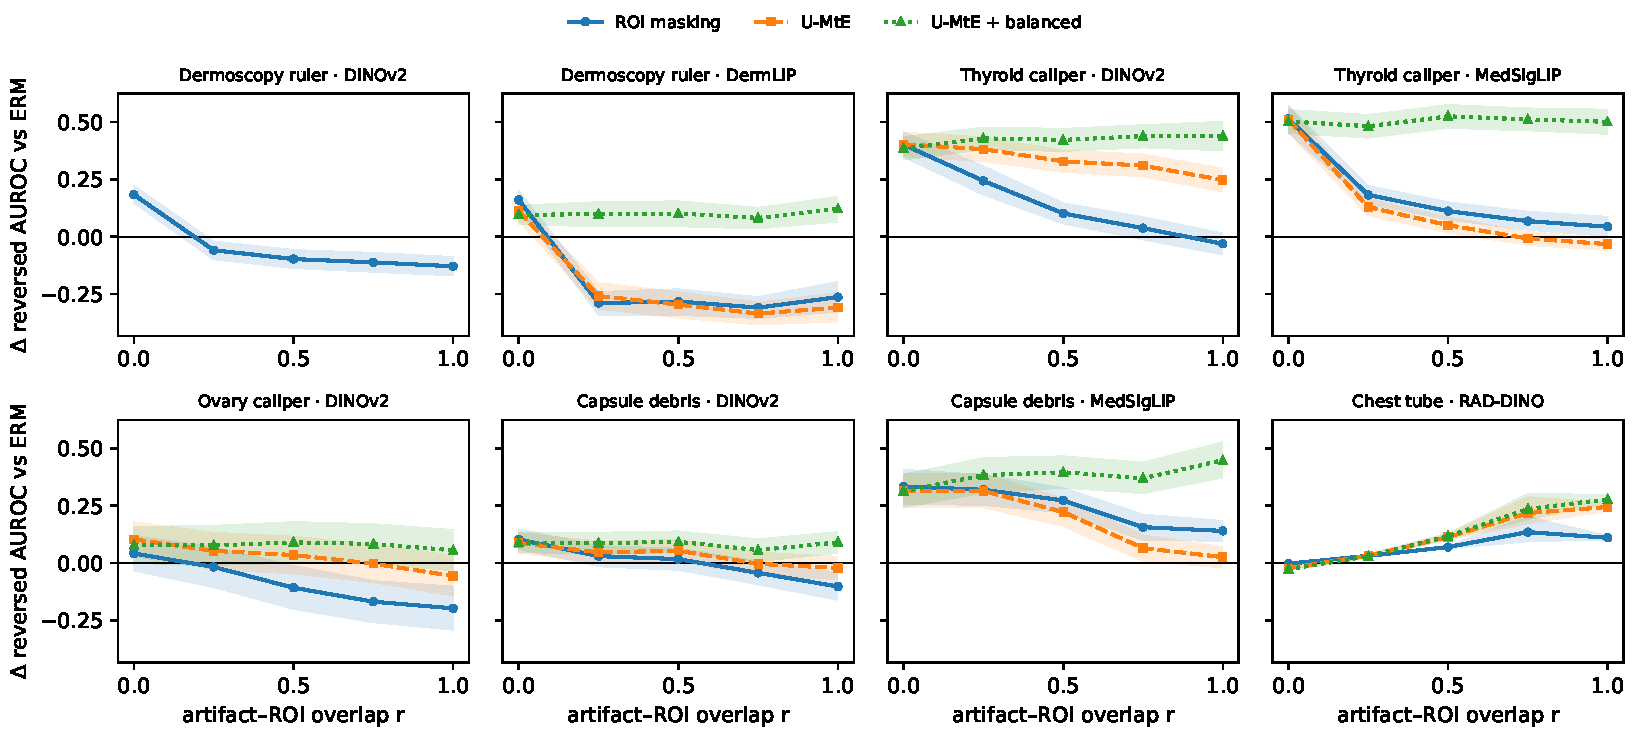
\includegraphics[width=\textwidth]{figures/dose_response.pdf}
\caption{Controlled overlap sweeps: change in reversed-test AUROC versus ERM as the synthetic artifact moves into the
ROI (95\% CIs shaded). ROI masking (blue) declines with overlap in every modality except chest radiography, where the
encoder ignores extra-pulmonary tubes; U-MtE with group balancing (green) is flat. Generated by
\texttt{scripts/make\_figures.py}.}\label{fig:dose}\end{figure*}

\subsection{Chest radiography: a boundary case}
With a synthetic tube swept into the lung fields of NIH pneumothorax radiographs (RAD-DINO), the encoder does not
use an extra-pulmonary tube at all (reversed 0.913 versus clean 0.915 at no overlap), so masking has nothing to
remove; inside the lungs the tube is used (reversed 0.614) and lung masking only partly removes it (0.725). On real
devices (RANZCR-CLiP linked to NIH; central lines and endotracheal tubes) masking helped for both locations. The
location-dependent \emph{harm} of masking is therefore not universal; what is universal in our data is that
masking leaves an in-ROI shortcut largely intact.

\section{Results: natural distribution, fine-tuning and label robustness}\label{sec:robust}

\subsection{Unaltered test distributions}
Without any resampling, in-ROI artifacts are naturally associated with the label in every cohort (thyroid calipers:
37.6\% of benign vs 24.1\% of malignant nodules; in-lesion hair: 31\% of melanomas vs 20\% of benign lesions;
capsule debris on the lesion: 23\% of polyp-like lesions vs 10\% of erosions). We trained on natural training data
and tested on untouched data: the official TN3K test split, each ISIC source held out in turn (a real change of
hospital and device), and held-out capsule frame blocks. On the shortcut-conflicting pairs, masking \emph{lowers}
AUROC for thyroid ($-0.102$ [$-0.139, -0.066$]) and for two of the three held-out hospitals (BCN $-0.016$
[$-0.027, -0.005$], MSK $-0.056$ [$-0.084, -0.029$]); it helps for HAM ($+0.053$) and does not differ significantly
from ERM on capsule. U-MtE with group balancing improves on masking for these pairs in every cohort in which it was
evaluated ($+0.014$ to $+0.065$) and gives the best or tied-best cross-group AUROC in three of five settings (HAM
0.786, BCN 0.734 vs 0.735, capsule 0.947); plain group balancing is best on thyroid and MSK. Without artifact labels,
U-MtE improves on masking for thyroid ($+0.051$) and HAM ($+0.023$) only.

\subsection{End-to-end fine-tuning}\label{sec:ft}
Fine-tuning ResNet-50 end-to-end (five folds) reproduces the frozen-backbone findings. Capsule: masking harms
in-ROI ($-0.284$ [$-0.347, -0.226$]) and helps out-of-ROI ($+0.301$), crossover $+0.584$ [$+0.469, +0.691$].
Thyroid: the crossover points the same way ($+0.057$ [$-0.021, +0.130$], five folds), and an end-to-end analogue of
U-MtE---an invariance penalty between masked images with and without a generic overlay---improves on masking by
$+0.143$ [$+0.099, +0.188$] without shortcut flipping (reversed 0.679, correlated 0.703), matching the best
label-using arm. It fails on capsule ($-0.021$), where the artifact resembles the pathology. Ovary (1,202 images)
is underpowered: U-MtE end-to-end has the best reversed, correlated and clean AUROC, with CIs overlapping masking.
A fine-tuned ViT-S reproduces the crossover on thyroid ($+0.168$ [$+0.074, +0.265$]), but the end-to-end U-MtE
analogue does not improve on masking with this architecture ($+0.009$ [$-0.021, +0.040$]).

\subsection{Robustness to artifact-label definitions}
Artifact masks for calipers come from a detector (visual audit: 95\% of thyroid detections lie on real calipers;
92--97\% of caliper-free images contain no visible caliper). Re-running the thyroid and ovary analyses with
large-marker-only ($\ge 50$ px) and strict-location ($r\ge0.7$ / $r<0.05$) definitions leaves the crossover
(thyroid $+0.215$ to $+0.262$; ovary $+0.170$ to $+0.195$) and the U-MtE$_{\text{protect}}$ gain over masking
(thyroid $+0.217$ to $+0.282$; ovary $+0.043$ to $+0.067$) significant in every variant; both grow under stricter
definitions, as expected if detector errors dilute rather than create the effects.

\section{Results: artifact-agnostic mask-then-erase}\label{sec:solution}

\begin{table*}[t]\centering\scriptsize
\caption{In-ROI artifacts (Trap~A): reversed-test AUROC, with min(reversed, correlated) in parentheses (penalises shortcut flipping). Best robust value per column in bold. Generated by \texttt{scripts/make\_main\_table.py}.}
\label{tab:main}
\begin{tabular}{llcccccccccc}
\toprule
Method & Needs & \rotatebox{90}{Hair/DINOv2} & \rotatebox{90}{Hair/DermLIP} & \rotatebox{90}{Thyroid/DINOv2} & \rotatebox{90}{Thyroid/MedSigLIP} & \rotatebox{90}{Thyroid/ConvNeXt} & \rotatebox{90}{Capsule/DINOv2} & \rotatebox{90}{Capsule/MedSigLIP} & \rotatebox{90}{Capsule/ConvNeXt} & \rotatebox{90}{Drain/RAD-DINO} & \rotatebox{90}{Drain/DINOv2} \\
\midrule
ERM & — & 0.49 (0.49) & 0.67 (0.67) & 0.29 (0.29) & 0.28 (0.28) & 0.35 (0.35) & 0.59 (0.59) & 0.59 (0.59) & 0.55 (0.55) & 0.19 (0.19) & 0.28 (0.28) \\
ROI masking & ROI & 0.45 (0.45) & 0.58 (0.58) & 0.40 (0.40) & 0.35 (0.35) & 0.36 (0.36) & 0.68 (0.68) & 0.70 (0.70) & 0.64 (0.64) & 0.24 (0.24) & 0.29 (0.29) \\
Mask + overlay augmentation & ROI & 0.46 (0.46) & – & 0.42 (0.42) & 0.38 (0.38) & 0.37 (0.37) & 0.70 (0.70) & 0.72 (0.72) & 0.65 (0.65) & 0.24 (0.24) & 0.29 (0.29) \\
\textbf{U-MtE (ours)} & ROI & 0.51 (0.51) & 0.51 (0.51) & 0.62 (0.62) & 0.55 (0.55) & 0.49 (0.49) & 0.57 (0.57) & 0.47 (0.47) & 0.56 (0.56) & 0.27 (0.27) & 0.28 (0.28) \\
\textbf{U-MtE, protected (ours)} & ROI + $Y$ of $A{=}0$ & 0.49 (0.49) & 0.59 (0.59) & 0.62 (0.62) & 0.61 (0.61) & 0.55 (0.55) & 0.67 (0.67) & 0.67 (0.67) & 0.64 (0.64) & 0.27 (0.27) & 0.28 (0.28) \\
Group-balanced & $A$ & 0.72 (0.72) & \textbf{0.81 (0.81)} & 0.68 (0.68) & 0.70 (0.70) & 0.66 (0.66) & 0.78 (0.78) & 0.81 (0.81) & 0.72 (0.72) & 0.54 (0.54) & 0.40 (0.40) \\
DFR & $A$ & \textbf{0.74 (0.74)} & 0.78 (0.78) & 0.74 (0.66) & 0.76 (0.72) & 0.71 (0.67) & 0.80 (0.80) & 0.80 (0.80) & 0.77 (0.77) & \textbf{0.68 (0.68)} & 0.55 (0.55) \\
Mask + DFR & ROI + $A$ & 0.69 (0.69) & – & 0.83 (0.74) & 0.81 (0.76) & 0.77 (0.72) & \textbf{0.88 (0.88)} & \textbf{0.90 (0.90)} & \textbf{0.86 (0.86)} & 0.65 (0.65) & \textbf{0.57 (0.57)} \\
\textbf{U-MtE + balanced (ours)} & ROI + $A$ & 0.70 (0.70) & 0.65 (0.65) & \textbf{0.79 (0.79)} & \textbf{0.79 (0.79)} & \textbf{0.74 (0.74)} & 0.86 (0.86) & 0.85 (0.85) & 0.80 (0.80) & 0.46 (0.46) & 0.44 (0.44) \\
\bottomrule
\end{tabular}
\end{table*}

\subsection{U-MtE repairs what masking leaves behind}
Without any artifact example, mask or label, U-MtE improves reversed AUROC over masking in the in-ROI regime of
every modality: thyroid calipers $+0.222$ [$+0.197, +0.251$] (DINOv2) and $+0.204$ [$+0.174, +0.237$] (MedSigLIP);
dermoscopic hair $+0.052$ [$+0.044, +0.062$]; synthetic capsule debris $+0.081$ [$+0.050, +0.112$]; synthetic
calipers $+0.278$ [$+0.232, +0.325$]; synthetic chest tubes $+0.134$ [$+0.120, +0.151$] (DINOv2 / RAD-DINO).
With MedSigLIP the unbalanced method \emph{loses} to masking in both controlled sweeps (debris $-0.114$
[$-0.147, -0.082$], calipers $-0.076$ [$-0.110, -0.043$]) although it wins on real thyroid calipers ($+0.204$);
the balanced variant beats masking in all four controlled sweeps ($+0.193$ to $+0.471$) and has no location
interaction in any of them. Disease protection turns the MedSigLIP debris failure into a gain ($+0.061$
[$+0.032, +0.092$] over masking) but not the caliper one ($-0.041$ [$-0.089, -0.005$]).

\subsection{Erasure, not augmentation}
Using the same generic overlays as training augmentation (overlaid copies of a random half of the training images,
in the masked view) gains at most $+0.03$ over masking; erasing their subspace instead gains $+0.207$
[$+0.182, +0.235$] (thyroid, DINOv2), $+0.177$ [$+0.148, +0.211$] (thyroid, MedSigLIP) and $+0.045$
[$+0.037, +0.054$] (hair) more than augmentation.

\subsection{When the artifact resembles the disease}
On real capsule debris U-MtE is worse than masking ($-0.115$): erosions carry yellow-white fibrin that resembles
debris, and a subspace estimated from real-debris templates is worse still ($-0.395$). Disease protection removes
the failure ($-0.010$ [$-0.020, -0.001$] generic, $-0.012$ [$-0.028, +0.003$] template) at a cost of at most
$0.012$ where erasure already works (thyroid $-0.005$ [$-0.036, +0.024$], hair $-0.012$ [$-0.020, -0.003$]).

\subsection{With image-level artifact labels}
Adding group balancing, U-MtE$_{\text{bal}}$ is the most robust model in thyroid ultrasound by the minimum of
correlated and reversed AUROC (0.788 DINOv2, 0.792 MedSigLIP; DFR 0.659 and 0.719); in real capsule endoscopy
masking plus last-layer retraining is higher (0.885 versus 0.857); on dermoscopic hair DFR alone is best (0.741)
because most of the hair shortcut is not in the hair pixels (removing every hair patch with the oracle mask gains
only $+0.015$). In both controlled sweeps the benefit of U-MtE$_{\text{bal}}$ no longer depends on location
(interaction $-0.000$ [$-0.023, +0.023$] capsule; $-0.054$ [$-0.098, -0.004$] thyroid), whereas that of masking
does ($+0.205$, $+0.432$).
The capsule findings replicate with MedSigLIP (crossover $+0.332$ [$+0.296, +0.365$]; masking plus DFR 0.901).
All thyroid and capsule findings replicate with a CNN (ConvNeXt-Base): crossovers $+0.284$ and $+0.292$; U-MtE $-$ mask $+0.128$ [$+0.112, +0.145$] and erase $-$ augment $+0.120$ [$+0.102, +0.139$] on thyroid.



\section{Discussion and limitations}
% Discussion — every number is taken from results/CROSS_COHORT.md, results/review2/* and the pre-registration result sections.
\paragraph{What the evidence supports} Masking is not a neutral preprocessing step: its benefit depends on where the
artifact sits. The strongest evidence is the real-artifact transplant, in which the same real calipers, hair or debris
on the same images are removed by masking outside the ROI and retained---with amplified reliance---inside it; the
real traps, covariate-matched traps, controlled sweeps, fine-tuned networks and foundation-model zero-shot scores all
point the same way. The claim is about the \emph{gap}. Whether in-ROI masking helps a little or harms depends on
whether the mask also removes disease context, which the linear-Gaussian account makes explicit and which differs
between modalities (harm in dermoscopy, small gains in ultrasound and capsule endoscopy).

\paragraph{Why this matters clinically} On the patient-disjoint official thyroid test split the in-ROI caliper is
associated with benign nodules; masking keeps it and removes competing evidence, and the malignant nodules that carry a
caliper are then missed more often at every operating point we examined. An ROI-masked model can therefore look
unchanged by overall AUROC while failing on exactly the cases in which the shortcut points the wrong way. Audits of
masked models should stratify performance by artifact presence and location.

\paragraph{Reading reversed-environment gains} A reversed-test gain can be manufactured by removing diagnosis-correlated
signal together with the artifact: erasure fitted on unpaired image-level labels and post-hoc prevalence recalibration
invert the correlated/reversed ordering. We report reversed, correlated and clean AUROC for every method and summarise
robustness by the minimum of correlated and reversed AUROC.

\paragraph{Limitations}
(i) \emph{Artifact labels.} Calipers are segmented by a rule-based detector and capsule debris by a patch-token probe
(IoU 0.62 against expert masks); hair masks are published semi-automatic masks. Our visual audits were carried out by
the analysis team, not by clinicians; an expert audit with two independent raters and inter-rater agreement is
prepared (blinded kit and scoring script in the repository) but not yet done. Label errors dilute the constructed
correlation and should bias effects toward zero, and stricter label definitions strengthen rather than weaken the
results (Sec.~\ref{sec:robustness}); the transplant experiment does not depend on the artifact-free group being
perfectly clean because the transplanted instance is identical at both locations.
(ii) \emph{Patient identifiers.} TN3K/TNCD, MMOTU and SEE-AI publish no patient or video identifiers for the pooled
images, so the trap splits group near-duplicates by perceptual hash and frame blocks (a stricter embedding grouping
leaves 11 of 12 primary estimates unchanged); the official TN3K/TNCD test split used for the unaltered-data analysis is
patient-disjoint. The one open cohort we found with patient identifiers, pathology labels and real calipers
(ThyUS2Path; 842 patients) has no nodule masks and uses a scanner interface on which our frozen caliper detector
fires on interface elements; external validation on it requires a transferred nodule segmentation and a re-validated
detector and is left for future work.
(iii) \emph{Constructed shifts.} Reversed environments are constructed by subsampling; real deployment shifts are
less extreme, which is why we report the unaltered test distributions separately.
(iv) \emph{Absolute performance.} Frozen encoders with linear heads are below the best published fine-tuned models on
the one cohort with a directly comparable benchmark (official TNCD split: 0.736 AUROC versus 0.773--0.784 for
fine-tuned CNNs with cross-entropy and up to 0.799 with curriculum learning, \citealp{gong2022acl}). The law
replicates with end-to-end fine-tuned networks in three of four cohorts; on ovarian ultrasound the fine-tuned ResNet-50
barely learns the task and shows no significant crossover (Sec.~\ref{sec:replication}). The other cohorts' binary
tasks have no published benchmark on the same split (Supplement~S10).
(v) \emph{Scope.} Chest radiography is a boundary case: the encoder ignored extra-pulmonary tubes and real drains carry
the shortcut through correlates. The linear-Gaussian account is fitted per model and cannot anticipate a shortcut
carried by correlates that the clean and correlated environments do not expose.
(vi) \emph{Pre-registration.} Every registration is committed before its outcome results (registry with commit hashes
and times in Supplement~S1); commit times are set by the committing machine, so only the registrations of the second
review round carry an external (GitHub push) time stamp, and the 16-test primary family was assembled after the
individual results.


\bibliographystyle{elsarticle-harv}
\bibliography{refs}
\end{document}
